\documentclass[12pt,compress,aspectratio=169]{beamer}

\usetheme{metropolis}
\setbeamersize{text margin left=.8cm,text margin right=.8cm}

\usefonttheme{professionalfonts}
\usepackage{amsmath,bm}
\usepackage{siunitx}
%\usepackage{graphicx}
\usepackage{tikz}
\usepackage{mathpazo}
\usepackage{xcolor,colortbl}
%\usepackage{hyperref}

\usetikzlibrary{patterns}

\setmonofont{Ubuntu Mono}
\setlength{\parskip}{0pt}
\setlength{\itemsep}{0pt}
\renewcommand{\baselinestretch}{1}

\sisetup{
  detect-all,
%  detect-display-math=true,%  <== NEWLY ADDED
%  detect-inline-family=math,% <== NEWLY ADDED
%  detect-inline-weight=math,% <== NEWLY ADDED
  number-math-rm=\mathnormal,
  per-mode=symbol
}

\title{Topic 6: Circular Motion}
\subtitle{Advanced Placement Physics C}
\author[TML]{Dr.\ Timothy Leung}
\institute{Olympiads School}
\date{July 21, 2020}

\newcommand{\pic}[2]{\includegraphics[width=#1\textwidth]{#2}}
\newcommand{\mb}[1]{\ensuremath\mathbf{#1}}
\newcommand{\eq}[2]{\vspace{#1}{\Large\begin{displaymath}#2\end{displaymath}}}


\begin{document}

\begin{frame}
  \maketitle
\end{frame}


\begin{frame}{Files to Download}
  Please download the following files from the school website if you have not
  already done so:
  \begin{itemize}
  \item\texttt{PhysAPC-06-circMotion-print.pdf}---The ``print version'' of the
    class slides for this topic.
  \item\texttt{PhysAPC-06-Homework.pdf}---Homework problems for this topic.
  \end{itemize}
  \vspace{.1in}Please download/print the PDF file for the class slides before
  each class. There is no point copying notes that are already on the slides.
  Instead, focus on things that aren't necessarily on the slides. If you wish
  to print the slides, we recommend printing 4 slides per page.
\end{frame}



\begin{frame}{Review of Circular Motion}
  In a \textbf{circular motion}, an object of mass $m$ moves in a circular path
  about a fixed center. In Grade 12 Physics, you should have studied
  \emph{uniform} circular motion, where:
  \begin{itemize}
  \item the object's speed (magnitude of velocity) is constant
  \item the object's \textbf{centripetal acceleration} is toward the center
  \item the object's acceleration is caused by a \textbf{centripetal force}
  \end{itemize}
\end{frame}



\section{Polar Coordinates}

\begin{frame}{Polar Coordinate System in 2D}
  \begin{columns}
    \column{.32\textwidth}
    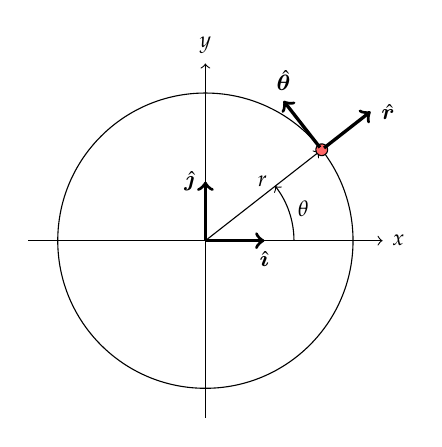
\begin{tikzpicture}[scale=.75]
      \draw[->](-3,0)--(3,0) node[pos=1,right]{\footnotesize$x$};
      \draw[->](0,-3)--(0,3) node[pos=1,above]{\footnotesize$y$};
      \draw[very thick,->](0,0)--(1,0)
      node[pos=1,below]{\footnotesize$\bm{\hat{\imath}}$};
      \draw[very thick,->](0,0)--(0,1)
      node[pos=1,left]{\footnotesize$\bm{\hat{\jmath}}$};
      \draw (0,0) circle(2.5);
      \begin{scope}[rotate=38]
        \draw[->] (0,0)--(2.45,0) node[midway,above]{\footnotesize$r$};
        \draw[fill=red!60] (2.5,0) circle(.1);
        \draw[very thick,->](2.55,0)--(3.55,0)
        node[pos=1,right]{\footnotesize$\hat{\bm{r}}$};
        \draw[very thick,->](2.5,.05)--(2.5,1.05)
        node[pos=1,above]{\footnotesize$\hat{\bm{\theta}}$};        
      \end{scope}
      \draw(1.5,0)[->] arc(0:38:1.5) node[pos=.55,right]{\footnotesize$\theta$};
    \end{tikzpicture}

    \column{.68\textwidth}
    In the Cartesian coordinate system, an object's position is described by
    its $x$ and $y$ coordinates:

    \eq{-.25in}{
      \mb{x}(t)=x(t)\bm{\hat{\imath}} + y(t) \bm{\hat{\jmath}}
      }

    \vspace{-.15in}For circular motion or general rotational motion, the
    \textbf{polar coordinate system} is preferred. The position of an object
    is described by:

    \eq{-.2in}{
      \mb{r}(t)=r(t)\hat{\bm{r}} + \theta(t)\hat{\bm{\theta}}
    }
    \begin{itemize}
    \item\vspace{-.15in}$r$ is distance from the origin
    \item $\theta$ is the standard angle, measured counter clockwise from the
      $x$ axis in \emph{radians}
    \end{itemize}
  \end{columns}
\end{frame}



\begin{frame}{Polar Coordinate System in 2D}
  \begin{columns}
    \column{.3\textwidth}
    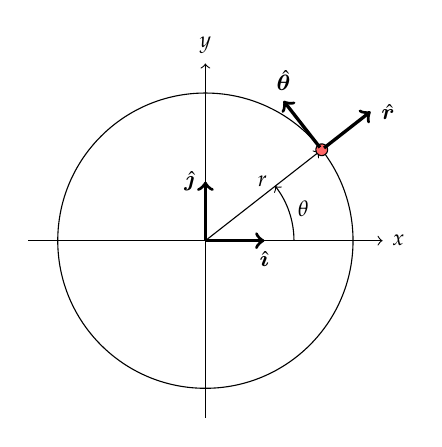
\begin{tikzpicture}[scale=.75]
      \draw[->](-3,0)--(3,0) node[pos=1,right]{\footnotesize$x$};
      \draw[->](0,-3)--(0,3) node[pos=1,above]{\footnotesize$y$};
      \draw[very thick,->](0,0)--(1,0)
      node[pos=1,below]{\footnotesize$\bm{\hat{\imath}}$};
      \draw[very thick,->](0,0)--(0,1)
      node[pos=1,left]{\footnotesize$\bm{\hat{\jmath}}$};
      \draw (0,0) circle(2.5);
      \begin{scope}[rotate=38]
        \draw[->] (0,0)--(2.45,0) node[midway,above]{\footnotesize$r$};
        \draw[fill=red!60] (2.5,0) circle(.1);
        \draw[very thick,->](2.55,0)--(3.55,0)
        node[pos=1,right]{\footnotesize$\hat{\bm{r}}$};
        \draw[very thick,->](2.5,.05)--(2.5,1.05)
        node[pos=1,above]{\footnotesize$\hat{\bm{\theta}}$};        
      \end{scope}
      \draw(1.5,0)[->] arc(0:38:1.5) node[pos=.55,right]{\footnotesize$\theta$};
    \end{tikzpicture}

    \column{.7\textwidth}
    \begin{itemize}
    \item Like the Cartesian system, the polar coordinate system is also
      right-handed
    \item Both basic vectors $\hat{\bm{r}}$ (radial direction) and
      $\hat{\bm{\theta}}$ (angular direction) rotate as the object moves
    \item Simpler way is to think of position as just two
      parameters, which is \emph{exactly} how position vectors are expressed in
      Grade 11/12 Physics: magnitude ($r$) and direction ($\theta$)!
    \item Cartesian and polar coordinates are related by:
      
      \vspace{-.35in}{\large
        \begin{align*}
          x&=r\cos\theta\\
          y&=r\sin\theta
        \end{align*}
      }
    \end{itemize}
  \end{columns}
\end{frame}



\begin{frame}{Cylindrical Coordinates in 3D}
  \begin{columns}
    \column{.45\textwidth}
    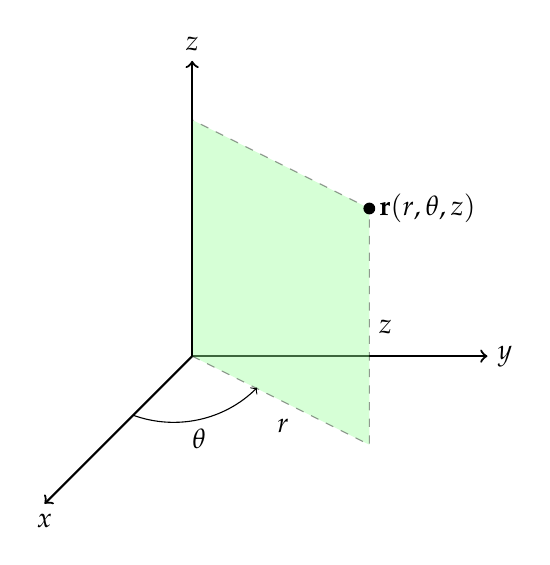
\begin{tikzpicture}[scale=.75]
      \draw[thick,->](0,0)--(-2.5,-2.5)node[pos=1,below]{$x$};
      \draw[thick,->](0,0)--(5,0)   node[pos=1,right]{$y$};
      \draw[dashed,fill=green!40,opacity=.4](0,0)--(3,-1.5)
      node[pos=.6,below left,opacity=1]{$r$}--(3,2.5)
      node[midway,right,black,opacity=1]{$z$}--(0,4);
      \fill[black](3,2.5) circle(.1) node[right]{$\mb{r}(r,\theta,z)$};
      \draw[->] (-1,-1) arc(-110:-45:2) node[midway,below]{$\theta$};
      \draw[thick,->](0,0)--(0,5) node[pos=1,above]{$z$};
    \end{tikzpicture}

    \column{.55\textwidth}
    One way to extend the coordinates coordinate system into 3D is the
    \textbf{cylindrical coordinate system}. Note that the discussions for this
    topic focuses on $xy$ plane. Since the $z$-axis is linearly independent of
    the $xy$ plane, motion along that direction is independent.
  \end{columns}
\end{frame}



\section{Rigid-Body Circular Motion}

\begin{frame}{Angular Position and Angular Velocity}
  \vspace{.2in}
  \begin{columns}
    \column{.32\textwidth}
    \begin{tikzpicture}[scale=.75]
      \draw[->](-3,0)--(3,0) node[pos=1,right]{\footnotesize$x$};
      \draw[->](0,-3)--(0,3) node[pos=1,above]{\footnotesize$y$};
      \draw (0,0) circle(2.5);
      \begin{scope}[rotate=38]
        \draw[->] (0,0)--(2.44,0) node[midway,above]{\footnotesize$r$};
        \draw[fill=red!60] (2.5,0) circle(.1);
      \end{scope}
      \draw(1,0)[->] arc(0:38:1) node[midway,right]{\footnotesize$\theta$};
    \end{tikzpicture}
    
    \column{.68\textwidth}
    For a constant $r$, the \textbf{angular position} $\theta$ determines an
    object's position as a function of time:
      
    \eq{-.2in}{
      \boxed{\theta=\theta(t)}
    }
    
    \textbf{Angular velocity} $\omega$ (or \textbf{angular frequency}) is its
    time derivative:
      
    \eq{-.2in}{
      \boxed{\omega(t)=\frac{d\theta(t)}{dt}=\dot{\theta}}
    }

    $\theta$ is measured in \si{radians}, and $\omega$ in \si{rad/\s}
  \end{columns}
\end{frame}



\begin{frame}{Velocity and Angular Velocity}
  \begin{columns}
    \column{.35\textwidth}
    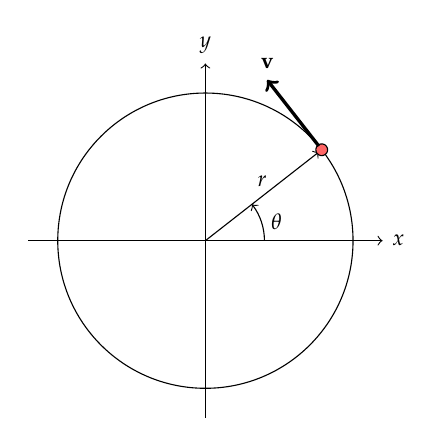
\begin{tikzpicture}[scale=.75]
      \draw[->](-3,0)--(3,0) node[pos=1,right]{\footnotesize$x$};
      \draw[->](0,-3)--(0,3) node[pos=1,above]{\footnotesize$y$};
      \draw (0,0) circle(2.5);
      \begin{scope}[rotate=38]
        \draw[->] (0,0)--(2.44,0) node[midway,above]{\footnotesize$r$};
        \draw[fill=red!60] (2.5,0) circle(.1);
        \draw[very thick,->](2.5,.08)--(2.5,1.5)
        node[pos=1,above]{\footnotesize$\mb{v}$};
      \end{scope}
      \draw(1,0)[->] arc(0:38:1) node[midway,right]{\footnotesize$\theta$};
    \end{tikzpicture}

    \column{.65\textwidth}
    The velocity of the object in circular motion is related to the angular
    velocity (or angular frequency) by:

    \eq{-.3in}{
      v=r\omega
    }    

    \begin{itemize}
    \item\vspace{-.25in} The direction of $\mb{v}$ is tangent to circle, along
      $\hat{\bm{\theta}}$, and therefore $\perp$ to $\hat{\bm{r}}$
    \item If $\omega>0$, the motion is counter-clockwise
    \item If $\omega<0$, the motion is clockwise
    \end{itemize}
  \end{columns}
\end{frame}



\begin{frame}{Velocity and Angular Velocity}
  \begin{columns}
    \column{.3\textwidth}
    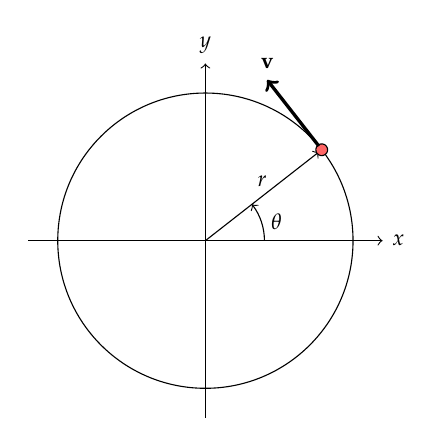
\begin{tikzpicture}[scale=.75]
      \draw[->](-3,0)--(3,0) node[pos=1,right]{\footnotesize$x$};
      \draw[->](0,-3)--(0,3) node[pos=1,above]{\footnotesize$y$};
      \draw (0,0) circle(2.5);
      \begin{scope}[rotate=38]
        \draw[->] (0,0)--(2.44,0) node[midway,above]{\footnotesize$r$};
        \draw[fill=red!60] (2.5,0) circle(.1);
        \draw[very thick,->](2.5,.08)--(2.5,1.5)
        node[pos=1,above]{\footnotesize$\mb{v}$};
      \end{scope}
      \draw(1,0)[->] arc(0:38:1) node[midway,right]{\footnotesize$\theta$};
    \end{tikzpicture}

    \column{.7\textwidth}
    The velocity of the object in circular motion is more properly related to
    the angular velocity using this vector cross product:

    \eq{-.25in}{
      \mb{v}=\bm{\omega}\times\mb{r}
    }

    \begin{itemize}
    \item\vspace{-.2in}$\bm{\omega}$: out of the page if motion is
      counter-clockwise
    \item $\bm{\omega}$: into the page if motion is clockwise
    \end{itemize}
    Visualizing $\bm{\omega}$ takes practice, but this vector notation is
    mathematically rigorious and consistent
  \end{columns}
\end{frame}



\begin{frame}{Period \& Frequency}
  \begin{columns}
    \column{.3\textwidth}
    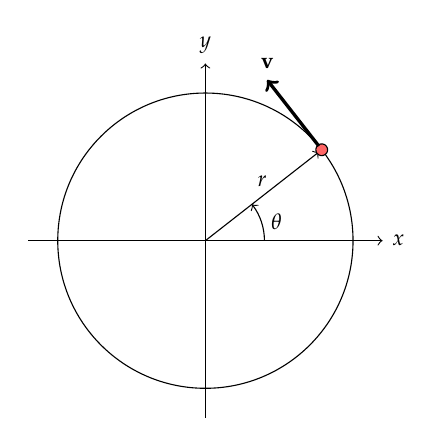
\begin{tikzpicture}[scale=.75]
      \draw[->](-3,0)--(3,0) node[pos=1,right]{\footnotesize$x$};
      \draw[->](0,-3)--(0,3) node[pos=1,above]{\footnotesize$y$};
      \draw (0,0) circle(2.5);
      \begin{scope}[rotate=38]
        \draw[->] (0,0)--(2.44,0) node[midway,above]{\footnotesize$r$};
        \draw[fill=red!60] (2.5,0) circle(.1);
        \draw[very thick,->](2.5,.08)--(2.5,1.5)
        node[pos=1,above]{\footnotesize$\mb{v}$};
      \end{scope}
      \draw(1,0)[->] arc(0:38:1) node[midway,right]{\footnotesize$\theta$};
    \end{tikzpicture}

    \column{.7\textwidth}
    For constant angular velocity $\omega$ (uniform circular motion), the
    motion is periodic. Its \textbf{frequency} and \textbf{period} are given by:

    \eq{-.15in}{
      f=\frac{\omega}{2\pi}\quad
      T=\frac{2\pi}{\omega}\quad
      f=\frac1T
    }
    
    $T$ is in \textbf{seconds} (\si{\s}) and $f$ is in \textbf{hertz}
    (\si{\hertz})
  \end{columns}
\end{frame}



\begin{frame}{Rotating Object Without Slipping}
  A tire with radius $r$ rolls along the road with an angular velocity $\omega$
  \emph{without slipping}. (This is a very common case for analysis.)  What
  is its velocity $v$
  \begin{enumerate}[a.]
  \item at the contact between the ground and the tire?
  \item at the center?
  \item at the top of the tire?
  \end{enumerate}

  \vspace{-.4in}
  \begin{center}
    \hspace{1in}
    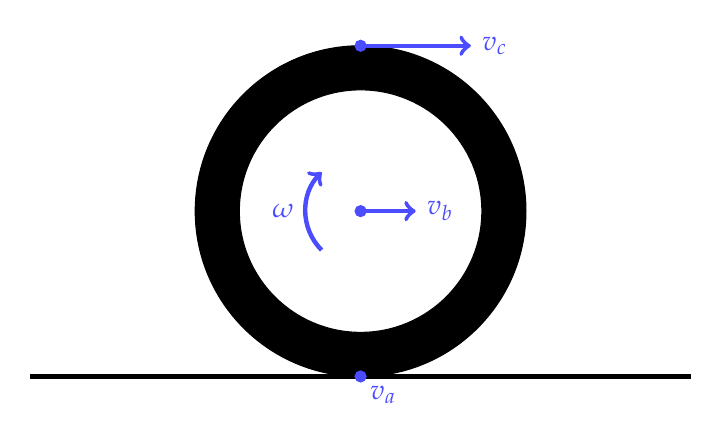
\begin{tikzpicture}[scale=.7]
      \draw[fill=black](0,0) circle(3);
      \draw[fill=white](0,0) circle(2.2);
      \draw[ultra thick](-6,-3)--(6,-3);
      \draw[ultra thick,blue!70,->](-.707,-.707) arc(225:135:1)
      node[midway,left]{$\omega$};
      \draw[fill=blue!70,blue!70](0,-3) circle(.1) node[below right]{$v_a$};
      \draw[fill=blue!70,blue!70](0,0) circle(.1);
      \draw[ultra thick,blue!70,->](0,0)--(1,0) node[pos=1,right]{$v_b$};
      \draw[fill=blue!70,blue!70](0,3) circle(.1);
      \draw[ultra thick,blue!70,->](0,3)--(2,3) node[pos=1,right]{$v_c$};
    \end{tikzpicture}
  \end{center}
\end{frame}



\begin{frame}{Angular Acceleration}
  The time derivative of $\omega$ is \textbf{angular acceleration}, which
  has a unit of \si{rad/\second^2}:

  \eq{-.2in}{
    \alpha=\dot{\omega}=\ddot{\theta}
  }

  Similar to the relationship between velocity and angular velocity,
  \textbf{tangential acceleration} $a_\theta$ is related to angular acceleration
  $\alpha$ by the radius $r$:
    
  \eq{-.2in}{
    a_\theta(t)=\dot{v}=r\dot{\omega}=r\alpha
  }
    
  For \emph{uniform} circular motion, $\omega$ is constant, and therefore
  $\alpha_\theta=0$
\end{frame}



\begin{frame}{With Calculus}
  Relationship between angular position and angular velocity:

  \eq{-.2in}{
    \omega(t)=\frac{d\theta}{dt}\quad\quad
    \theta(t)=\int\omega(t) dt +\theta_0
  }

  Relationship between angular velocity and angular acceleration:

  \eq{-.2in}{
    \alpha(t)=\frac{d\omega}{dt}=\frac{d^2\theta}{dt^2}
    \quad\quad\omega(t)=\int\alpha(t) dt+\omega_0
  }

  The relationships are the same as in rectilinear motion.
\end{frame}




\begin{frame}{Kinematics in the Angular Direction}
  For constant $\alpha$, the kinematic equations are just like in rectilinear
  motion:

  \vspace{-.3in}{\Large
    \begin{align*}
      \theta&=\theta_0 + \omega_0 t + \frac{1}{2}\alpha t^2\\
      \theta&=\theta_0+ \frac{\omega_0+\omega}{2} t\\
      \omega^2& = \omega_0^2+ 2\alpha(\theta-\theta_0)
    \end{align*}
  }
  
  If $\alpha$ is \emph{not} constant, integration will be required.
\end{frame}



\begin{frame}{A Simple Example}
  \textbf{Example 1:} An object moves in a circle with angular acceleration
  \SI{3.}{rad/\s^2}. The radius is \SI{2.}{\metre} and it starts from rest. How
  long does it take for this object to finish a circle?
\end{frame}



\begin{frame}{Centripetal Acceleration \& Centripetal Force}
  There is also a component of acceleration toward the center of the motion,
  called the \textbf{centripetal acceleration} $a_r$:

  \eq{-.15in}{
    \boxed{\mb{a}_r=-\frac{v^2}{r}\hat{\bm{r}}=-\omega^2r\hat{\bm{r}}}
  }

  (The negative sign is because $\mb{\hat{r}}$ is radially outward from the
  center.) The force that causes the centripetal acceleration is called the
  \textbf{centripetal force}:

  \eq{-.15in}{
    \boxed{\mb{F}_r=m\mb{a}_r=-\frac{mv^2}{r}\hat{\bm{r}}}
  }
\end{frame}



\begin{frame}{Centripetal Acceleration for Uniform Circular Motion}
  In uniform circular motion ($\alpha=0$) problems where the period or
  frequency are known, the speed of the object is:

  \eq{-.15in}{
    v=\frac{2\pi r}{T}=2\pi rf
  }

  Centripetal acceleration can therefore be expressed based on $T$ or $f$:

  \eq{-.2in}{
    \mb{a}_r=-\frac{v^2}{r^2}\hat{\bm{r}}\quad\rightarrow\quad
    \boxed{
      \mb{a}_r=-\frac{4\pi^2r}{T^2}\hat{\bm{r}}=-4\pi^2rf^2\hat{\bm{r}}
    }
  }
\end{frame}



\begin{frame}{Acceleration: The General Case}
  \begin{columns}
    \column{.2\textwidth}
    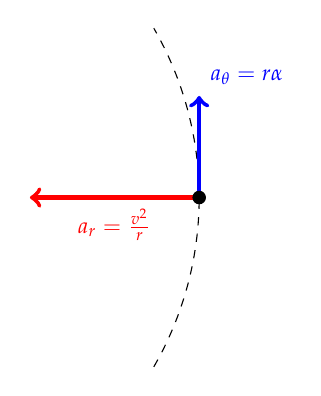
\begin{tikzpicture}[scale=4.3]
      \draw[dashed] (.866,-.5) arc(-30:30:1);
      \draw[ultra thick, red,->] (1,0)--(.5,0)
      node[pos=0.5,below]{\footnotesize $a_r=\frac{v^2}{r}$};
      \draw[ultra thick, blue,->] (1,0)--(1,.3)
      node[pos=1,above right]{\footnotesize $a_\theta=r\alpha$};
      \fill (1,0) circle(.02);
    \end{tikzpicture}
    
    \column{.8\textwidth}
    \begin{itemize}
    \item In general circular motion, there are two components of acceleration:
      \begin{itemize}
      \item\textcolor{red}{\textbf{Centripetal acceleration} $a_r$} depends on
        radius of curvature $r$ and instantaneous speed $v$. The direction of
        the acceleration is toward the center of the circle.
      \item \textcolor{blue}{\textbf{Tangential acceleration} $a_\theta$}
        depends on radius $r$  and angular acceleration $\alpha$. The direction
        of the acceleration is tangent to the circle
      \end{itemize}
    \end{itemize}
  \end{columns}

  \vspace{.2in}Most of the cases in AP Physics are uniform circular motion.
\end{frame}



\begin{frame}{How to Solve Circular Motion Problems}
  \begin{enumerate}
  \item Is there any circular motion?
  \item If so, the condition for circular motion is:

    \eq{-.2in}{
      \mb{F}_\mathrm{provided}=\mb{F}_\mathrm{required}
    }
    \begin{itemize}
    \item\vspace{-.2in}The \emph{provided} force comes from FBD
    \item The \emph{required} force comes from the centripetal force equation 
    \end{itemize}
  \item If the net force also has a tangential component, then there is also
    a change in angular velocity
  \end{enumerate}
\end{frame}



\begin{frame}{Example: Horizontal Motion}
  \begin{columns}
    \column{.4\textwidth}
    \pic{1}{puck-on-table.png}
    
    \column{.6\textwidth}
    \textbf{Example 2:} In the figure on the left, a mass
    $m_1=\SI{3.}{\kilo\gram}$ is rolling around a frictionless table with
    radius $R=\SI{1.}{\metre}$. with a speed of \SI{2.}{\metre\per\second}.
    What is the mass of the weight $m_2$?
  \end{columns}
\end{frame}



\begin{frame}{Banked Curves on Highways and Racetracks}
  \begin{columns}
    \column{.35\textwidth}
    \centering
    \pic{.8}{banked-turn-acceleration.png}\\
    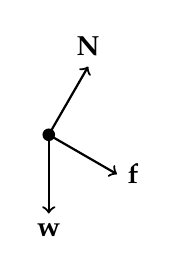
\begin{tikzpicture}
      \fill[black](0,0) circle(.08);
      \draw[thick,->,rotate=-30](0,0)--(0,1)node[pos=1,above]{$\mb{N}$};
      \draw[thick,->](0,0)--(0,-1)node[pos=1,below]{$\mb{w}$};
      \draw[thick,->,rotate=60](0,0)--(0,-1)node[pos=1,right]{$\mb{f}$};
    \end{tikzpicture}
    \begin{tikzpicture}
      \draw[->](0,0)--(1,0) node[pos=1,right]{$x$};
      \draw[->](0,0)--(0,1) node[pos=1,above]{$y$};
    \end{tikzpicture}

    \column{.65\textwidth}
    No motion in the $y$ direction, i.e.\ no net force:

    \eq{-.35in}{
      \sum F_y=N\cos\theta-f\sin\theta-w=0
    }

    Net force in the $x$ direction is the centripetal force:

    \eq{-.35in}{
      \sum F_x=N\sin\theta +f\cos\theta = \frac{mv^2}{r}
    }

    Friction force $\mb{f}$ may be static or kinetic.
  \end{columns}
\end{frame}



\begin{frame}{Banked Curves on Highways and Racetracks}
  \begin{columns}
    \column{.35\textwidth}
    \centering
    \pic{.8}{banked-turn-acceleration.png}\\
    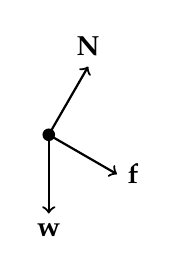
\begin{tikzpicture}
      \fill[black](0,0) circle(.08);
      \draw[thick,->,rotate=-30](0,0)--(0,1)node[pos=1,above]{$\mb{N}$};
      \draw[thick,->](0,0)--(0,-1)node[pos=1,below]{$\mb{w}$};
      \draw[thick,->,rotate=60](0,0)--(0,-1)node[pos=1,right]{$\mb{f}$};
    \end{tikzpicture}
    \begin{tikzpicture}
      \draw[->](0,0)--(1,0) node[pos=1,right]{$x$};
      \draw[->](0,0)--(0,1) node[pos=1,above]{$y$};
    \end{tikzpicture}

    \column{.65\textwidth}
    For analysis, use the simplified equation for friction $f=\mu N$ (i.e.\
    assume either kinetic friction or maximum static friction), and weight
    $w=mg$, the equations on the previous slides can be arranged as:

    \vspace{-.4in}{\Large
      \begin{align*}
        N\left(\cos\theta-\mu\sin\theta\right) &=mg\\
        N\left(\sin\theta+\mu\cos\theta\right) &=\frac{mv^2}{r}
      \end{align*}
    }
  \end{columns}
\end{frame}


\begin{frame}{Banked Curves on Highways and Racetracks}
  \begin{columns}
    \column{.35\textwidth}
    \centering
    \pic{.8}{banked-turn-acceleration.png}\\
    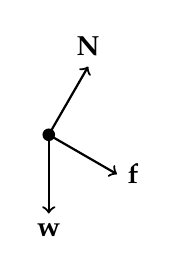
\begin{tikzpicture}
      \fill[black](0,0) circle(.08);
      \draw[thick,->,rotate=-30](0,0)--(0,1)node[pos=1,above]{$\mb{N}$};
      \draw[thick,->](0,0)--(0,-1)node[pos=1,below]{$\mb{w}$};
      \draw[thick,->,rotate=60](0,0)--(0,-1)node[pos=1,right]{$\mb{f}$};
    \end{tikzpicture}
    \begin{tikzpicture}
      \draw[->](0,0)--(1,0) node[pos=1,right]{$x$};
      \draw[->](0,0)--(0,1) node[pos=1,above]{$y$};
    \end{tikzpicture}

    \column{.65\textwidth}
    Dividing the two equations removes both the normal force and mass terms:

    \eq{-.15in}{
      \frac{\sin\theta+\mu\cos\theta}{\cos\theta-\mu\sin\theta}
      =\frac{v^2}{rg}
    }

    The \emph{maximum} velocity $v_{\textrm{max}}$ can be expressed as:

    \eq{-.25in}{
      \boxed{v_{\textrm{max}}=
        \sqrt{rg\frac{\sin\theta+\mu\cos\theta}{\cos\theta-\mu\sin\theta}}
      }
    }

    Note that $v_\mathrm{max}$ does not depend on mass.
  \end{columns}
\end{frame}



\begin{frame}{Banked Curves on Highways and Racetracks}
  In the limit of $\mu=0$ (frictionless case), the equation reduces to:

  \eq{-.1in}{
    \boxed{ v_{\textrm{max}}=\sqrt{rg\tan\theta} }
  }

  And in the limit of a flat roadway with no banking ($\theta=0$,
  $\sin\theta=0$ and $\cos\theta=1$), the equation reduces to:

  \eq{-.2in}{
    \boxed{
      v_{\textrm{max}}=\sqrt{\mu rg}
    }
  }
\end{frame}




%
%
%\begin{frame}{Another Example: Exit Ramp}
%  \textbf{Example 3:} A car exits a highway on a ramp that is banked at
%  \ang{15} to the horizontal. The exit ramp has a radius of curvature of
%  \SI{65}{\metre}. If the conditions are extremely icy and the driver cannot
%  depend on any friction to help make the turn, at what speed should the driver
%  travel so that the car will not skid off the ramp? What if there is friction?
%\end{frame}


\section{Vertical Circles}

\begin{frame}{Vertical Circles}
  Circular motion with a horizontal path is straightforward. However, for
  vertical motion:
  \begin{itemize}
  \item Generally difficult to solve by dynamics and kinematics
  \item Instead, use conservation of energy to solve for $\mb{v}$
  \item Then use the equation for centripetal force to find other forces
  \end{itemize}

  \textbf{Remember:} If it is impossible to get the required centripetal
  force, then it could not continue the circular motion
\end{frame}



\begin{frame}{What About a Pendulum?}
  A simple pendulum is also like a vertical circular motion problem.

  \vspace{.1in}\begin{columns}
    \column{.35\textwidth}
    \begin{tikzpicture}[scale=.8]
      \fill[pattern=north east lines] (-1,0) rectangle (1,0.2);
      \draw[very thick](-1,0)--(1,0);
      \begin{scope}[rotate=20]
        \draw[thick](0,0)--(0,-5);
        \tikzstyle{balloon}=[ball color=red!70!black];
        \shade[balloon] (0,-5) circle (0.2) node[below right]{$m$};
        \draw[->,very thick,red!70!black](0,-5)--(0,-3.3)
        node[pos=1,left]{\footnotesize $\mb{T}$};
        \draw[->,very thick,red!70!black,rotate around={-20:(0,-5)}](0,-5)--(0,-6.5)
        node[pos=1,below]{\footnotesize $\mb{w}$};
      \end{scope}
      \draw[dashed,thin](0,0)--(0,-5);
      \draw[dashed,thin](3.54,-3.54) arc(315:225:5);
      \draw[->](0,-2) arc(270:290:2) node[pos=0.5,below]{$\theta$};
    \end{tikzpicture}

    \column{.65\textwidth}
    \begin{itemize}
    \item There are two forces act on the pendulum: weight $\mb{w}=m\mb{g}$, and
    tension $\mb{T}$
    \item Speed of the pendulum at any height is found using conservation
      of energy
      \begin{itemize}
      \item Tension $\mb{T}$ is always $\perp$ to motion, therefore it doesn't
        do any work
      \item Work is done by gravity (a conservative force) alone
      \end{itemize}
    %\item The velocity vector is tangent to the path
    \item Tangential and centripetal accelerations are based on the net force
      along the angular and radial directions
    \end{itemize}
  \end{columns}
\end{frame}



\begin{frame}{Simple Pendulum}
  At the top of the swing, velocity $v$ is zero, therefore:
  
  \vspace{.1in}\begin{columns}
    \column{.5\textwidth}
    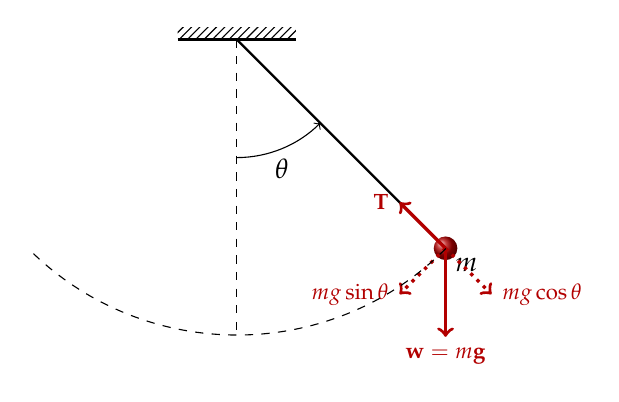
\begin{tikzpicture}[scale=.75]
      \fill[pattern=north east lines] (-1,0) rectangle (1,0.2);
      \draw[very thick](-1,0)--(1,0);
      \begin{scope}[rotate=45]
        \draw[thick](0,0)--(0,-5);
        \tikzstyle{balloon}=[ball color=red!70!black];    
        \shade[balloon] (0,-5) circle (0.2) node[below right]{$m$};
        \draw[dotted,->,very thick,red!70!black](0,-5)--(-1.1,-5)
        node[pos=1,left]{\footnotesize $mg\sin\theta$};
        \draw[dotted,->,very thick,red!70!black](0,-5)--(0,-6.1)
        node[pos=1,right]{\footnotesize $mg\cos\theta$};
        \draw[->,very thick,red!70!black](0,-5)--(0,-3.9)
        node[pos=1,left]{\footnotesize $\mb{T}$};
        \draw[->,very thick,red!70!black,rotate around={-45:(0,-5)}](0,-5)--(0,-6.5)
        node[pos=1,below]{\footnotesize $\mb{w}=m\mb{g}$};
      \end{scope}
      \draw[dashed,thin](0,0)--(0,-5);
      \draw[dashed,thin](3.54,-3.54) arc(315:225:5);
      \draw[->](0,-2) arc(270:315:2) node[pos=.5,below]{$\theta$};
    \end{tikzpicture}

    \column{.5\textwidth}
    Centripetal acceleration is also zero:

    \eq{-.2in}{
      a_r=\frac{v^2}{r}=0
    }

    and therefore the net force along the radial direction $\hat{\bm{r}}$ is
    zero. The tension force $T$ can be calculated:

    \eq{-.2in}{
      T=mg\cos\theta
    }
  \end{columns}
  At the highest point when $\theta$ is largest, tension is the lowest.
\end{frame}



\begin{frame}{Simple Pendulum}
  In the radial direction $\hat{\bm{\theta}}$, there is still a net force of
  $mg\sin\theta$, therefore:
  \begin{columns}
    \column{.5\textwidth}
    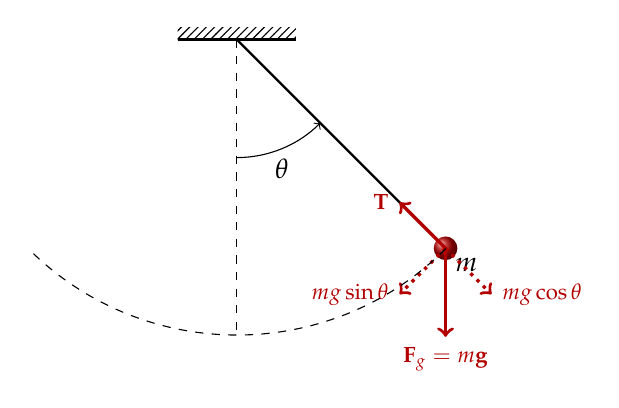
\begin{tikzpicture}[scale=.75]
      \fill[pattern=north east lines] (-1,0) rectangle (1,0.2);
      \draw[very thick](-1,0)--(1,0);
      \begin{scope}[rotate=45]
        \draw[thick](0,0)--(0,-5);
        \tikzstyle{balloon}=[ball color=red!70!black];    
        \shade[balloon] (0,-5) circle (0.2) node[below right]{$m$};
        \draw[dotted,->,very thick,red!70!black](0,-5)--(-1.1,-5)
        node[pos=1,left]{\footnotesize $mg\sin\theta$};
        \draw[dotted,->,very thick,red!70!black](0,-5)--(0,-6.1)
        node[pos=1,right]{\footnotesize $mg\cos\theta$};
        \draw[->,very thick,red!70!black](0,-5)--(0,-3.9)
        node[pos=1,left]{\footnotesize $\mb{T}$};
        \draw[->,very thick,red!70!black,rotate around={-45:(0,-5)}](0,-5)--(0,-6.5)
        node[pos=1,below]{\footnotesize $\mb{F}_g=m\mb{g}$};
      \end{scope}
      \draw[dashed,thin](0,0)--(0,-5);
      \draw[dashed,thin](3.54,-3.54) arc(315:225:5);
      \draw[->](0,-2) arc(270:315:2) node[pos=.5,below]{$\theta$};
    \end{tikzpicture}

    \column{.5\textwidth}
    There is a tengential acceleration along $\hat{\bm{\theta}}$, with a
    magnitude of:

    \eq{-.25in}{
      a_\theta=g\sin\theta
    }

    \vspace{-.1in}This is the same acceleration as an object sliding down a
    frictionless ramp at an angle of $\theta$.
  \end{columns}
\end{frame}



\begin{frame}{Simple Pendulum}
  At the bottom of the swing, the velocity is at its maximum value,
  
  \vspace{.1in}\begin{columns}
    \column{.35\textwidth}
    \begin{tikzpicture}[scale=.8]
      \fill[pattern=north east lines] (-1,0) rectangle (1,0.2);
      \draw[very thick](-1,0)--(1,0);

      \draw[thick](0,0)--(0,-5);
      \tikzstyle{balloon}=[ball color=red!70!black];    
      \shade[balloon] (0,-5) circle (0.2) node[below right]{$m$};
      \draw[->,very thick,red!70!black](0,-5)--(0,-2.5)
      node[pos=1,right]{\footnotesize $\mb{T}$};
      \draw[->,very thick,red!70!black](0,-5)--(0,-6.5)
      node[pos=1,below]{\footnotesize $\mb{w}=m\mb{g}$};

      \draw[dashed,thin](0,0)--(0,-5);
      \draw[dashed,thin](3.54,-3.54) arc(315:225:5);
    \end{tikzpicture}

    \column{.65\textwidth}
    \begin{itemize}
    \item Maximum centripetal acceleration:

      \eq{-.25in}{
        a_r=\frac{v^2}{r}
      }
    \item No tangential acceleration:

      \eq{-.25in}{
        a_\theta=0
      }
    \item At the lowest point, tension is the highest:

      \eq{-.3in}{
        T=w+F_r=m\left(g+\frac{v^2}{r}\right)
      }
    \end{itemize}
  \end{columns}
\end{frame}



\begin{frame}{Example Problem}
  \textbf{Example 4:} You are playing with a yo-yo with a mass of
  \SI{225}{\gram}. The full length of the string is \SI{1.2}{\metre}. You
  decide to see how slowly you can swing it in a vertical circle while keeping
  the string fully extended, even when the yo-yo is at the top of its swing.
  \begin{enumerate}[A.]
  \item Calculate the minimum speed at which you can swing the yo-yo while
    keeping it on a circular path.
  \item Find the tension in the string when the yo-yo is at the side and at the
    bottom of its swing. 
  \end{enumerate}
\end{frame}



\begin{frame}{Example Problem}
  \textbf{Example 5:} A cord is tied to a pail of water, and the pail is swung
  in a vertical circle of \SI{1.}{\metre}. What must be the minimum velocity of
  the pail be at its highest point so that no water spills out?

  \begin{enumerate}[(a)]
  \item\SI{3.1}{\metre\per\second}
  \item\SI{5.6}{\metre\per\second}
  \item\SI{20.7}{\metre\per\second}
  \item\SI{100.5}{\metre\per\second}
  \end{enumerate}
\end{frame}



\begin{frame}{Example: Roller Coaster}
  \textbf{Example 6:} A roller coaster car is on a track that forms a circular
  loop, of radius $R$, in the vertical plane. If the car is to maintain contact
  with the track at the top of the loop (generally considered to be a good
  thing), what is the minimum speed that the car must have at the bottom of the
  loop. Ignore air resistance and rolling friction.
  \begin{enumerate}[(a)]
  \item $\sqrt{2gR}$
  \item $\sqrt{3gR}$
  \item $\sqrt{4gR}$
  \item $\sqrt{5gR}$
  \end{enumerate}
\end{frame}



\begin{frame}{Example}
  \textbf{Example 7:} A stone of mass $m$ is attached to a light strong string
  and whirled in a \emph{vertical} circle of radius $r$. At the exact bottom of
  the path, the tension of the string is three times the weight of the stone.
  The stone's speed at that point is given by:
  \begin{enumerate}[(a)]
  \item $2\sqrt{gR}$
  \item $\sqrt{2gR}$
  \item $\sqrt{3gR}$
  \item $4gR$
  \end{enumerate}
\end{frame}



%\section{Torque}
%
%\begin{frame}{Torque and Rotational Equilibrium}
%  Let's consider this question:
%  \begin{center}
%    \fbox{
%      \begin{minipage}{.7\textwidth}
%        Two people stand on a board of uniform density. One person has a mass of
%        \SI{50}{\kilo\gram} and stands \SI{10}{\metre} away from the fulcrum
%        (pivot). The second person has a mass of \SI{65}{\kilo\gram}. How far
%        away from the fulcrum would the second person have to stand for the
%        system to have to be in equilibrium?
%      \end{minipage}
%    }
%  \end{center}
%\end{frame}
%
%
%
%\begin{frame}{Equation of Motion}{Newton's Second Law}
%  Recall Newton's second law of motion for objects with constant mass:
%    
%  \eq{-.2in}{
%    \mb{F}_\mathrm{net}=m\mb{a}
%  }
%  \begin{itemize}
%  \item Is it also true for \emph{circular} motion?
%  \item If a net force $\mb{F}_\mathrm{net}$ causes a mass to accelerate
%    (linearly), what causes a mass to go into circular motion?
%  \end{itemize}
%
%  \uncover<2->{
%    \vspace{.3in}
%    \textbf{Answer:} We need to introduce a few concepts first\ldots
%  }
%\end{frame}
%
%
%
%\begin{frame}{Torque}
%  I have a rod on a table, and with my fingers, I push the two ends of the rod
%  with equal force $\textcolor{red}{F}$. \textbf{What happens?}
%  \begin{center}
%    \begin{tikzpicture}[scale=1.5]
%      \fill[black!75,draw=black,thick] (-2,-.15) rectangle (2,.15);
%      \draw[ultra thick,red,->](-1.8,-.7)--(-1.8,-.15) node[pos=0,below]{$F$};
%      \draw[ultra thick,red,->]( 1.8, .7)--( 1.8, .15) node[pos=0,above]{$F$};
%    \end{tikzpicture}
%  \end{center}
%  $\mb{F}_\mathrm{net}=\mb{0}$, therefore $\mb{a}=\mb{0}$. But (obviously) it
%  won't stay still either!
%\end{frame}
%
%
%
%\begin{frame}{What is Torque?}
%  \textbf{Torque} (or \textbf{moment}) is the tendency for a force to change
%  the rotational motion of a body.
%  
%  \begin{itemize}
%  \item A force $\mb{F}_a$ acting at a point some distance $\mb{r}$ (called the
%    \textbf{moment arm}) from a \textbf{fulcrum} (or \textbf{pivot}) at an angle
%    $\phi$ between $\mb{F}_a$ and $\mb{r}$
%  \item e.g.\ the force to twist a screw
%%  \item In the example below, an applied force $\mb{F}_a$ is applied away from
%%    the pivot at an angle $\phi$. This generates a torque around the pivot.
%  \end{itemize}
%  \begin{center}
%    \begin{tikzpicture}[scale=2.5]
%      \fill[black!75,draw=black!75] (0,-.1) rectangle (2,.1);
%      \fill[black!75,draw=black,thick] (0,0) circle (.2);
%      \fill[black] (0,0) circle (.03);
%      \draw[ultra thick,red,->](0,0)--(1.8,0) node[midway,below]{$\mb{r}$};
%      \draw[ultra thick,blue,->](1.2,-.7)--(1.8,0)node[pos=0,below]{$\mb{F}_a$};
%      \draw[ultra thick,->] (1.4,0) arc(180:229:.4)
%      node[midway,left]{$\phi$};
%    \end{tikzpicture}
%  \end{center}
%\end{frame}
%
%
%
%\begin{frame}{Torque}
%  In scalar form, we can express torque $\bm{\tau}$ as the force $\mb{F}_a$,
%  the \textbf{moment arm} $\mb{r}$ and the angle $\phi$ between $\mb{F}_a$ and
%  $\mb{r}$:
%
%  \eq{-.2in}{
%    \boxed{\tau=rF_a\sin\phi}
%  }
%  
%  In vector form, we use the cross-product:
%
%  \eq{-.2in}{
%    \boxed{\bm{\tau}=\mb{r}\times\mb{F}_a}
%  }
%  \begin{center}
%    \begin{tabular}{l|c|c}
%      \rowcolor{pink}
%      \textbf{Quantity} & \textbf{Symbol} & \textbf{SI Unit} \\ \hline
%      Torque        & $\bm{\tau}$ & \si{\newton\metre} \\
%      Applied force & $\mb{F}_a$  & \si{\newton} \\
%      Moment arm (from fulcrum to force) & $\mb{r}$ & \si{\metre}\\
%      Angle between force and moment arm & $\phi$ & (no units)
%    \end{tabular}
%  \end{center}
%\end{frame}
%
%
%
%\begin{frame}{Torque}
%  Going back to the example question:
%  \begin{center}
%    \begin{tikzpicture}
%      \fill[black!75,draw=black!75] (-5,-.05) rectangle (5,.05);
%      \fill (0,0) circle (.1);
%      \draw[ultra thick](0,0)--(.5,-1.5)--(-.5,-1.5)--(0,0);
%      \uncover<2->{
%        \draw[ultra thick,red!75,->](0,0)--(-4.8,0) node[pos=.5,below]{$d_1$};
%        \draw[ultra thick,red!75,->](-4.8,0)--(-4.8,-1)node[pos=1,below]{$F_1$};
%      }
%      \uncover<3->{
%        \draw[ultra thick,blue!60,->](0,0)--(4,0) node[pos=.5,below]{$d_2$};
%        \draw[ultra thick,blue!60,->](4,0)--(4,-1.2) node[pos=1,below]{$F_2$};
%      }
%    \end{tikzpicture}
%  \end{center}
%  \begin{itemize}
%  \item<2->$F_1$ will rotate the board counter clockwise
%  \item<3->$F_2$ will rotate the board clockwise
%  \item<4->The beam will remain static (in equilibrium) if
%
%    \eq{-.2in}{ F_1d_1=F_2d_2 }
%  \end{itemize}
%\end{frame}
%
%
%
%\begin{frame}{Rotational Equilibrium}
%  An object is in \textbf{translational equilibrium} is when the force acting
%  it is zero, and therefore the acceleration of its center of mass is zero:
%  
%  \eq{-.2in}{
%    \mb{F}=\mb{0}
%  }
%
%  \vspace{-.15in}Likewise, an object is in \textbf{rotational equilibrium} when
%  the net torque acting on it is zero, which means that the angular momentum at
%  its center of mass is constant:
%
%  \eq{-.3in}{
%    \bm{\tau}=\mb{0}
%  }
%
%  \vspace{-.1in}Note that it does \emph{not} mean that the object has no
%  rotational motion; it just means that the object's overall
%  \emph{rotational state} is not changing, i.e.\ $\alpha=0$
%\end{frame}
%
%
%
%\begin{frame}{Example Problem}
%  \textbf{Example 8a:} Find the net torque on point C.
%
%  \vspace{-.2in}
%  \begin{center}
%    \begin{tikzpicture}[scale=2.5]
%      \fill[blue!40!white,draw=black,thick] (-1.65,-.15) rectangle (1.65,.15);
%      \draw[thick,<->](-1.5,-.5)--(1.5,-.5) node[midway,below]{\SI{3.}{m}};
%      \draw[thick,<->](-1.5,.5)--(0,.5) node[midway,below]{\SI{1.5}{m}};
%      \draw[dashed,thick](-2.5,0)--(2.5,0);
%      \draw[dashed,thick](0,.5)--(0,-.5);
%      \draw[ultra thick,orange,->](0,0)--(1,1)node[pos=1,right]{\SI{30}{N}};
%      \draw[thick,->](0,.4)arc(90:45:.4)
%      node[pos=.7,above]{\footnotesize\ang{45}};
%      \draw[ultra thick,orange,->](-1.5,0)--(-2.3,-.46)
%      node[pos=1,left]{\SI{20}{\newton}};
%      \draw[thick,->](-1.9,0) arc(180:210:.4)
%      node[midway,left]{\footnotesize\ang{30}};
%      \draw[ultra thick,orange,->](1.5,0)--(2,-.29)
%      node[pos=1,right]{\SI{10}{\newton}};
%      \draw[thick,->](1.9,0) arc(0:-30:.4)
%      node[midway,right]{\footnotesize\ang{30}};
%      \fill[black,draw=black,thick] (-1.5,0) circle(.1);
%      \fill[black,draw=black,thick] (   0,0) circle(.1);
%      \fill[black,draw=black,thick] ( 1.5,0) circle(.1);
%      \node(A) at (-1.5,0) {\color{white}\textbf{A}};
%      \node(B) at (0,0) {\color{white}\textbf{B}};
%      \node(C) at (1.5,0) {\color{white}\textbf{C}};
%    \end{tikzpicture}
%  \end{center}
%  \uncover<2->{
%    \textbf{Example 8b:} Now find the net torque on A.
%  }
%\end{frame}
%
%
%
%\section{Angular Momentum}
%
%\begin{frame}{Angular Momentum}
%  \vspace{.15in}
%  \begin{columns}
%    \column{.77\textwidth}
%    Consider a mass $m$ connected to a massless beam rotates with speed $v$ at
%    a distance $r$ from the center (shown on the right). It has an
%    \textbf{angular momentum} ($L$) of
%    
%    \eq{-.2in}{
%      \boxed{\mb{L}=\mb{r}\times\mb{p}}
%    }
%    
%    \vspace{-.1in}Expanding the terms in the definition:
%    
%    \eq{-.4in}{
%      \mb{L}=\mb{r}\times(m\mb{v})=m\mb{r}\times(\bm{\omega}\times\mb{r})
%      =mr^2\bm{\omega}
%    }
%    
%    \vspace{-.2in}Which gives us:
%    
%    \eq{-.3in}{
%      \boxed{\mb{L}=I\bm{\omega}}
%    }
%    
%    \vspace{-.2in}The quantity $I$ is called the \textbf{moment of inertia}.
%    
%    \column{.23\textwidth}
%    \begin{tikzpicture}[scale=2.5]
%      \begin{scope}[rotate=70]
%        \fill[black!75,draw=black!75] (0,-.02) rectangle (2,.02);
%        \fill[blue!75,draw=blue,thick] (2,0) circle(.05);
%        \node(M) at (2,-.2) {$m$};
%        \fill[black] (0,0) circle (.05);
%        \draw[ultra thick,red,->](0,0)--(2,0)node[pos=.5,right]{$\mb{r}$};
%        \draw[ultra thick,->](2,0)--(2,.5)node[pos=1,above]{$\mb{v}$};
%      \end{scope}
%    \end{tikzpicture}
%  \end{columns}
%\end{frame}
%
%
%
%\begin{frame}{Moment of Inertia}
%  A single particle:
%  
%  \eq{-.2in}{
%    \boxed{I=r^2m}
%  }
%
%  A collection of particles:
%
%  \eq{-.2in}{
%    \boxed{I=\sum r_i^2m_i}
%  }
%
%  Continuous distribution of mass:
%
%  \eq{-.2in}{
%    \boxed{I=\int r^2dm}
%  }
%\end{frame}
%
%
%
%\begin{frame}{Moment of Inertia}
%  \begin{center}
%    \pic{.7}{mic.png}
%  \end{center}
%\end{frame}
%
%
%
%\begin{frame}{Angular Momentum and Moment of Inertia}
%  \begin{itemize}
%  \item Linear and angular momentum have very similar expressions
%    
%    \eq{-.2in}{
%      \mb{p}=m\mb{v}\quad\quad\quad \mb{L}=I\bm{\omega}
%    }
%  \item Just as $\mb{p}$ describes the overall \emph{translational} state of a
%    physical system, $\mb{L}$ describes its overall \emph{rotational} state
%  \item Momentum of inertia $I$ can be considered to be an object's
%    ``rotational mass''
%  \end{itemize}
%\end{frame}
%
%
%
%\begin{frame}{Newton's Second Law of Motion}{For Rotational Motion}
%  \eq{-.35in}{
%    \bm{\tau}=\mb{r}\times\mb{F}=\mb{r}\times\frac{d\mb{p}}{dt}
%    =\frac{d(\mb{r}\times\mb{p})}{dt}\;\;\longrightarrow\;\;
%%      \tau=rF=rm\frac{dv}{dt}=\frac{d(rmv)}{dt}\quad\longrightarrow\quad
%%    \end{displaymath}
%%    \begin{displaymath}
%    \boxed{\bm{\tau} =\frac{d\mb{L}}{dt}}
%  }
%  \begin{itemize}
%  \item If the net torque on a system is zero, then the rate of change
%    of angular momentum is zero, and we say that the angular momentum is
%    conserved. 
%  \item e.g.\ When an ice skater starts to spin and draws his arms inward.
%    Since angular momentum is conserved, a decrease in $r$ means an
%    increase in $\omega$.
%  \end{itemize}
%\end{frame}
%
%
%
%\begin{frame}{Newton's Second Law of Motion}
%  {Comparing Translational and Rotational Motion}
%  Newton's second law of motion for rotational motion has a very similar
%  form to translational motion:
%
%  \eq{-.2in}{
%    \mb{F}=\frac{d\mb{p}}{dt}\quad\quad\bm{\tau}=\frac{d\mb{L}}{dt}
%  }
%
%  For objects with constant mass (translational motion) or constant moment of
%  inertia (rotational motion), Newton's second law reduces to:
%
%  \eq{-.2in}{
%    \mb{F}=m\mb{a}\quad\quad \bm{\tau}=I\bm{\alpha}
%  }  
%\end{frame}
%
%
%
%\begin{frame}{But there is no rotational motion, is there?}
%  Even when there is no apparent rotational motion, it does not mean that
%  angular momentum is zero! In this case, mass $m$ travels along a straight
%  path at constant velocity (uniform motion), but the angular momentum around
%  point $P$ is not zero:
%  \begin{center}
%    \begin{tikzpicture}
%      \draw[dashed](-5,0)--(5,0);
%      \draw[very thick,red!70!black,->](-5,0)--(-3,0)
%      node[pos=1,below]{$\mb{v}$};
%      \tikzstyle{balloon}=[ball color=red!70!black];
%      \shade[balloon] (-5,0) circle(.2) node[above left,red!70!black]{$m$};
%      \fill[black] (0,-2) circle(.05) node[below]{$P$};
%      \draw[very thick,blue!70!black,->](0,-2)--(-5,0)
%      node[midway,below left]{$\mb{r}$};
%      \uncover<2->{
%        \draw[dotted](0,0) circle(.2) node[above left]{$m$};
%        \draw[thick,red!50,->](.2,0)--(2,0)node[pos=1,right]{$\mb{v}$};
%        \draw[thick,blue!50,->](0,-2)--(0,0) node[midway,left]{$\mb{r}$};
%      }
%      \uncover<3->{
%        \draw[dotted](4,0) circle(.2) node[above left]{$m$};
%        \draw[thick,red!50,->](4.2,0)--(6,0)node[pos=1,right]{$\mb{v}$};
%        \draw[thick,blue!50,->](0,-2)--(4,0)node[midway,above left]{$\mb{r}$};
%      }
%    \end{tikzpicture}
%  \end{center}
%  \uncover<4>{
%    Since there is no force and no torque acting on the object, both the linear
%    momentum ($\mb{p}=m\mb{v}$) and angular momentum
%    ($\mb{L}=\mb{r}\times\mb{v}$) are constant.
%  }
%\end{frame}
%
%
%
%\begin{frame}{Example Problem}
%  \textbf{Example 9:} A skater extends her arms (both arms!), holding a
%  \SI{2.}{\kilo\gram} mass in each hand. She is rotating about a vertical axis
%  at a given rate. She brings her arms inward toward her body in such a way that
%  the distance of each mass from the axis changes from \SI{1.}{\metre} to
%  \SI{.50}{\metre}. Her rate of rotation (neglecting her own mass) will?
%\end{frame}
%
%
%
%\begin{frame}{Last Example}
%  \textbf{Example 10:} A \SI{1.}{\kilo\gram} mass swings in a vertical circle
%  after having been released from a horizontal position with zero initial
%  velocity. The mass is attached to a massless rigid rod of length
%  \SI{1.5}{\metre}. What is the angular momentum of the mass, when it is in its
%  lowest position?
%\end{frame}
%
%
%
%\section{Rotational Kinetic Energy}
%
%\begin{frame}{Rotational Kinetic Energy}
%  To find the kinetic energy of a rotating system of particles (discrete number
%  of particles, or continuous mass distribution), we sum (or integrate) the
%  kinetic energy of the individual particles:
%    
%  \vspace{-.3in}{\Large
%    \begin{align*}
%      K&=\sum_i\frac{1}{2}m_iv_i^2=\frac{1}{2}\left(\sum_i m_ir_i^2\right)\omega^2\\
%      K&=\int\frac{1}{2}v^2dm=\frac{1}{2}\left(\int r^2dm\right)\omega^2
%    \end{align*}
%  }
%  
%  It's no surprise that in both case, rotational kinetic energy is given by:
%  
%  \eq{-.25in}{
%    \boxed{K=\frac{1}{2}I\omega^2}
%  }
%\end{frame}
%
%
%
%\begin{frame}{Kinetic Energy of a Rotating System}
%  The total kinetic energy of a rotating system is the sum of its translational
%  and rotational kinetic energies at its center of mass:
%
%  \eq{-.2in}{
%    \boxed{K=\frac{1}{2}mv_\mathrm{CM}^2+\frac{1}{2}I_\mathrm{CM}\omega^2}
%  }
%  
%  In this case, $I_\mathrm{CM}$ is calculated at the center of
%  mass. For simple problems, we only need to compute rotational kinetic energy
%  at the pivot:
%
%  \eq{-.2in}{
%    \boxed{K=\frac{1}{2}I_\mathrm{P}\omega^2}
%  }
%  
%  In this case, the $I_\mathrm{P}$ is calculated at the pivot.
%  \textbf{IMPORTANT:} $I_\mathrm{CM}\neq I_\mathrm{P}$
%\end{frame}
%
%
%
%\begin{frame}{Parallel Axis Theorem}
%  \begin{columns}
%    \column{.35\textwidth}
%    \pic{1}{Steiner.png}
%    
%    \column{.65\textwidth}
%    The \textbf{parallel axis theorem} relates the moment of inertia of an
%    object along two different but parallel axis by:
%
%    \eq{-.2in}{
%      \boxed{I=I_{\textrm{CM}}+md^2}
%    }
%  \end{columns}
%\end{frame}
\end{document}
